\chapter{Heading North}

The winter retreat that year lasted for the two months of January and
February. This was the first time I had lived at Amaravati. I was
invited to stay in a room often used by visiting senior sangha members,
which meant that although the weather outside was cold and miserable, I
was warm and comfortable, for which I was very grateful.

Although the accommodation and routine were agreeable, my mind was
preoccupied with what I imagined might lie ahead at Harnham. Amaravati
and Chithurst were sister monasteries in more ways than one. Regular
exchanges of residents took place between the two communities, and they
were both run by the English Sangha Trust. The monastery at Harnham was
managed by a completely separate and independent body, these days called
\href{https://ratanagiri.org.uk/about/organization}{\underline{Harnham
Buddhist Monastery Trust}} {[}86{]}.

I had visited Harnham monastery before, and I confess I found the
buildings and the surrounding countryside somewhat bleak. That might
have been because my visits coincided with the Kathina season which
always falls in autumn. Whatever the reasons for my reservations, that
retreat period gave me plenty of time to look and feel into where, when
and how I was creating suffering out of something that I was only
imagining. Perhaps it would all be wonderful, with a community of monks,
novices and anagarikas living in a cooperative manner, with attentive
trustees supporting the sangha -- all in an effort to create something
profoundly beautiful. Of course, I didn't know.

Thankfully, part way through that retreat, I came to realize that many
of my worries were a result of the way I held the idea of leadership. I
have written in
\href{https://forestsangha.org/teachings/books/servant-of-reality?language=English}{\emph{\underline{Servant}}
\emph{\underline{of Reality}}}, {[}87{]} (p2) about how, one morning,
while reflecting on the words of our morning chanting, \emph{I am a
servant of the Buddha, I am a servant of the Dhamma, I am a servant of
the Sangha,} a fresh perspective on the idea of leadership opened up.

A wonderful feeling of relief came over me as I recognized how appealing
I found the suggestion of being a servant. And how different holding
that image in my mind felt, compared to the idea of being a master. It
was obvious that I really didn't want to be a master. I began to see the
extent to which I had been struggling to try and master everything:
trying to master my meditation, master my relationships, master my
understanding of Dhamma. It was just deluded personality yet again,
trying to control everything. I started to realize that not only did I
not want to be a master, but nobody had ever told me that I had to be
one. I could be a servant if I wished. With this recognition, a burden
fell away. The unconscious commitment to compulsively controlling was
seen just a little bit more clearly. My vision of Harnham, and whatever
the future might hold, was transformed.

Being a leader of a community is a way of serving that community; it is
not merely a way of controlling it. This change in perspective helpfully
influenced how I would navigate the vicissitudes of community life over
the following years.

There never had been any good reason for concern about what I would find
when I arrived at Harnham. Amongst the six or so residents living there
at the time was one with whom I was already somewhat acquainted. Tan
Suriyo I had known as Robin when he was an anagarika at Chithurst and
was my driver and chaperone on a number of occasions. He took monks'
Precepts at the same time as Tan Puñño, and I had the good fortune of
being their mentor during the period of transition from anagarika to
monk. There was also a particularly helpful anagarika from Boston,
called Chris (these days known as Ajahn Jayanto). Tan Suriyo and he were
from a similar part of America, and they each contributed to an
atmosphere of goodness and integrity. Sometimes I imagine that in the
future scientists will develop a way of measuring an individual's
integrity, similar to how these days they measure intelligence. Maybe in
the future IQ will stand for Integrity Quotient. I estimate these two
men would score very highly.

Another unexpected and agreeable aspect of the move was finding that
there was a Dhamma Hall building project well underway. The nitty-gritty
work of excavation and outer construction was virtually all complete,
and the building was now ready for the next, thoroughly pleasing, phase
of interior design. It could hardly have been a more welcome task. Of
course it wasn't without its challenges. The first decision to be taken
was regarding a large bay window that had been planned to sit behind the
main shrine. From what I had learned in consultations at Chithurst,
according to the Chinese concept of \emph{feng shui}, there should never
be a window behind a Buddha image. I cannot substantiate that in any
way; however, the sense I have of how it would feel to be looking at a
Buddha image with trees and possibly even people moving in the
background, is not one of stillness. When I look at a shrine I want to
feel stilled. So I took the decision to cancel the bay window project
and had the construction workers continue building the wall all the way
up, but leaving an opening on top for an atrium, so light would descend
down from above the Buddha. The decision wasn't met with the approval of
everybody but I was unwavering. Nearly thirty years later, and I am
still convinced it was the right decision. We don't go into a spiritual
sanctuary in order to gaze outside at the view.

T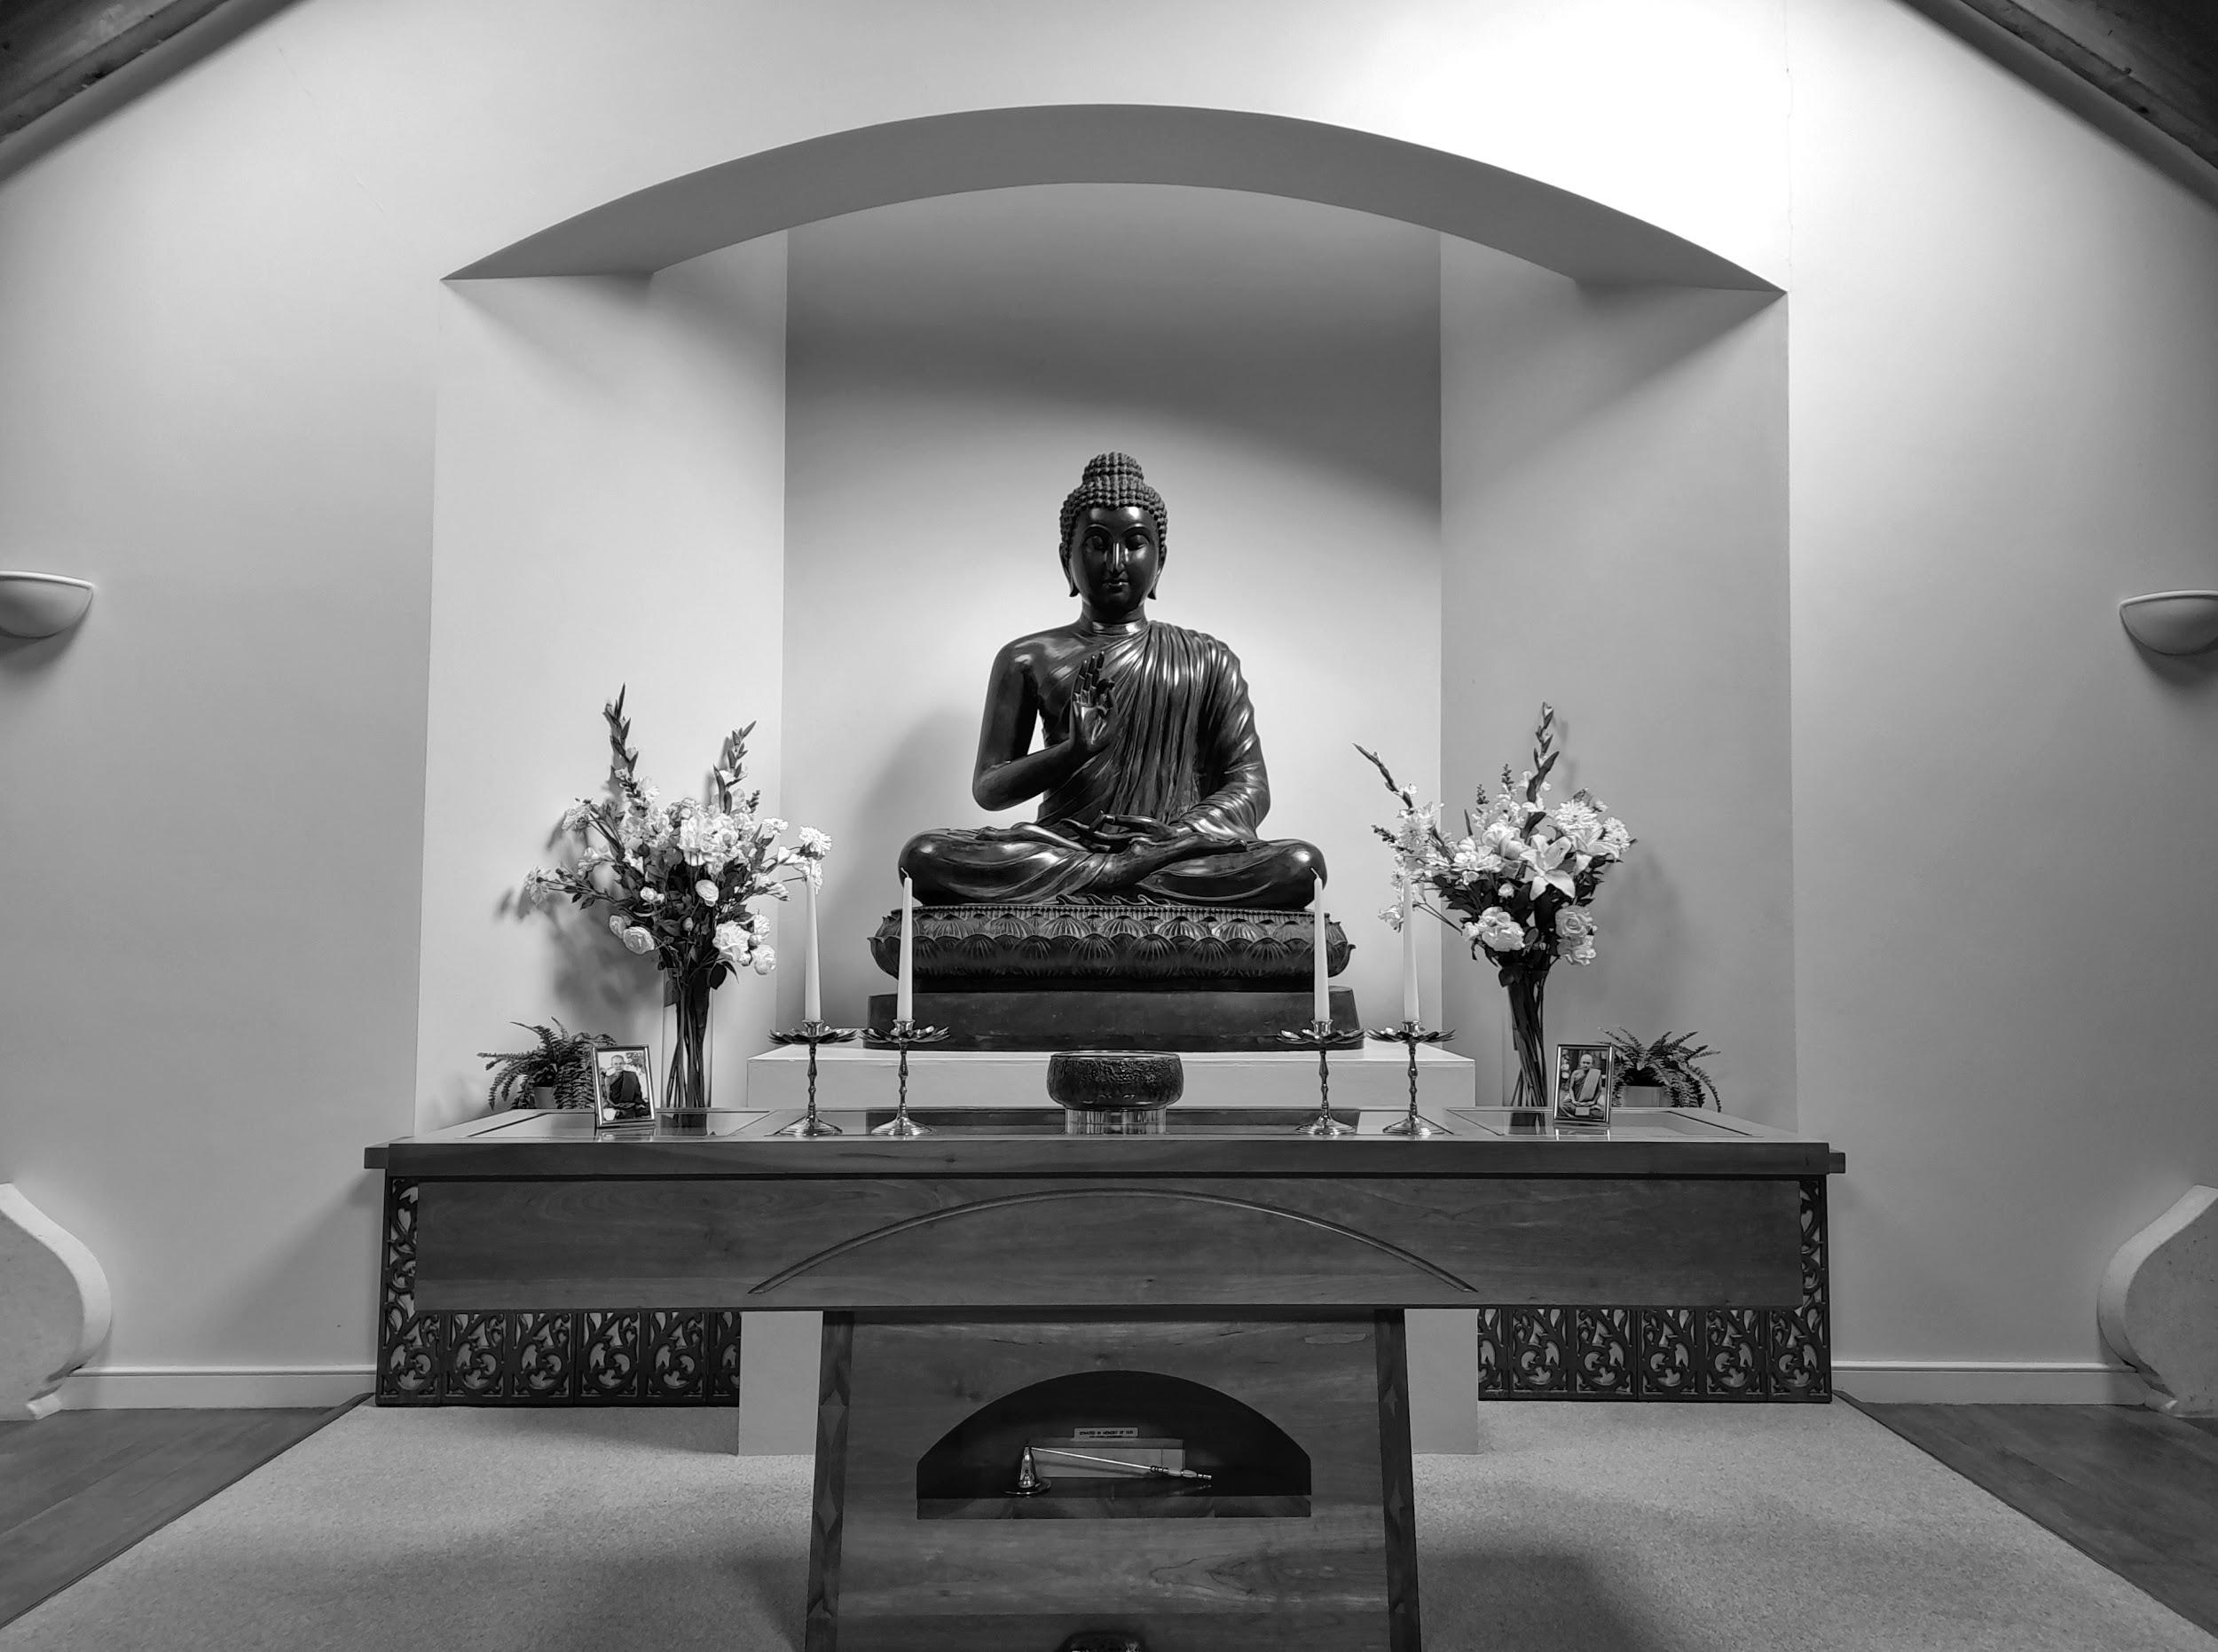
\includegraphics[width=3.35278in,height=2.48125in]{media/image7.jpeg}an
Vipassi and I considered very carefully how we should approach the
period of my taking over as leader. The previous abbot, Ajahn Pabakharo,
as mentioned earlier, had been a helicopter pilot during the war in
Vietnam. He was a tall and imposing figure. He spoke with a commanding
sense of what was needed, and seemed to relish any opportunity to use a
chainsaw. He and I could hardly have been more different.
Understandably, it was going to take time for the resident sangha to get
used to the style of this new leaner, quieter Kiwi abbot; also, the
trustees would have to get used to yet another way of doing things. I
was the fifth senior incumbent in the ten years the monastery had been
running. Tan Vipassi and I decided that we wouldn't change anything that
wasn't necessary for the first six months: just observe and wait until
we had a good enough overall impression of the place and its people.
That decision worked well. As the weeks and months went by, a new
configuration of community dynamics was emerging, building work
proceeded without too many hiccups, and everyone seemed to be
cooperating well.

The month of May in that first year marked approximately ten years since
Harnham Monastery had begun, and it felt fitting to have some sort of
celebration. The occasion was modest but rewarding and I am pleased we
did it. I was also pleased that the ceremony we organized later that
year in September to celebrate establishing a \emph{sima} boundary
inside the new Dhamma Hall went so well.

Senior sangha members from various monasteries down south were invited.
Eight handsome bodhi leaf-shaped `\emph{sima} markers' were carved by a
local craftsman, along with eight large and very heavy stone spheres
that were used in the formal designation of the \emph{sima} boundaries.
As at Chithurst, we went through the process of removing any possible
previous \emph{sima} boundary, and then established the new one. It was
conducted with an attitude of dignity and respect as befits such an
occasion.

It was also later in that first year, 1991, that the main
\emph{Buddha-rupa} for the Dhamma Hall arrived. When Ajahn Pabakharo was
still abbot, he had made arrangements for it to be cast in Thailand, and
it was sponsored by a long-time \emph{looksit} (disciple) of Tan Ajahn
Chah's, Khun Siri. On receiving notification that a half-metric-ton
image was due to arrive, no small amount of trepidation was triggered
within me. Over the years I had seen many large Buddha images that were
far from inspiring to look at. The image that was about to arrive would
grace our Dhamma Hall for ever; whatever it was, was what we would be
bowing to from now on. Ideally, of course, one would be making an effort
to maintain equanimity, but \emph{upekkha} is a virtue in which I was,
and still sadly am, undeveloped. I wanted our Dhamma Hall to be a space
in which the Thais, Burmese, Sri Lankans and Westerners, would all feel
uplifted when they entered. If the central Buddha rupa on the shrine
looked garish and out of proportion, that was going to be difficult. I
assume I knew enough about practice back then to appreciate that wanting
was not the problem, it was clinging to wanting which led to suffering,
but I wasn't able to let go. I \emph{really, really} wanted it to be
inspiring, so I suffered accordingly.

On opening the crate, I saw that my concerns were, once again,
groundless. The bronze Buddha image had been superbly crafted and cast;
because of the unpolished finish, it had a slight green patina, the
colour of the moss on the stone walls. Immediately upon seeing it I was
relieved. \emph{Anumodana} Khun Siri and everyone else who was involved
in making this offering. For my part, I continue to work on developing
equanimity.

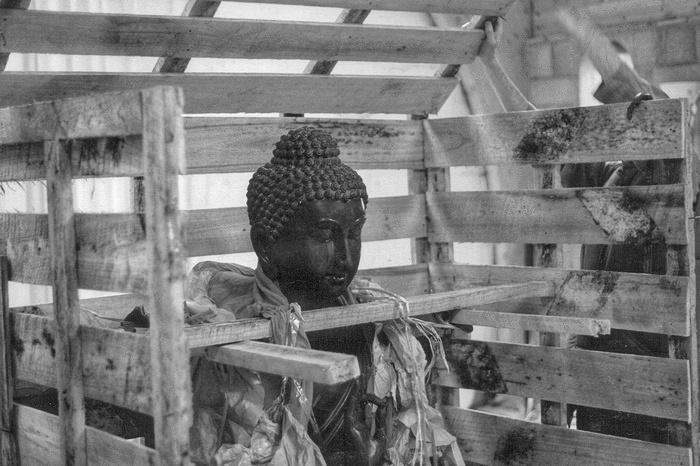
\includegraphics[width=3.67569in,height=2.46319in]{media/image8.jpeg}

